\documentclass{standalone}
\usepackage{tikz}

\newcommand\polygon[3][]{
  \pgfmathsetmacro{\angle}{360/#2}
  \pgfmathsetmacro{\startangle}{-90 + \angle/2}
  
  \begin{scope}[#1]
    \foreach \i in {1,2,...,#2} {
      \pgfmathsetmacro{\x}{\startangle + \angle*\i}
      \coordinate (p\i) at (\x:1 cm);
    }
    % Preenche o polígono com a cor especificada
    \fill[#3] (p1)
      \foreach \i in {2,3,...,#2} {
        -- (p\i)
      } -- cycle;

    \draw[#3,line width=.5pt,color=black] (p1)
      \foreach \i in {2,3,...,#2} {
        -- (p\i)
      } -- cycle;
      
    % Desenha as linhas como antes
    \foreach \i in {1,2,...,#2} {
      \foreach \j in {\i,...,#2} {
        %\draw[black,line width=.4pt] (p\i) -- (p\j);
      }
    }
  \end{scope}
}

\begin{document}
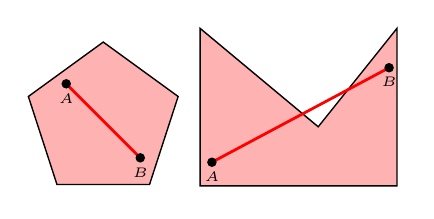
\begin{tikzpicture}
  %\draw (-1,-1) grid (10,10);
  \polygon{5}{red!30}
  \draw[line width=1pt, red] (-.47,.47) -- (.47,-.47);
  \draw[fill] (-.47,.47) circle (1.5pt) node[below] {\tiny$A$};
  \draw[fill] (.47,-.47) circle (1.5pt) node[below] {\tiny$B$};
  %\polygon[xshift=2.2cm]{6}{red!30}
  %\polygon[xshift=4.4cm]{7}{red!30}
  %\polygon[xshift=6.6cm]{8}{red!30}

\begin{scope}[xshift=35pt,yshift=-23.5pt]
\coordinate (a) at (0,0);
\coordinate (b) at (0,2);
\coordinate (c) at (1.5,0.75);
\coordinate (d) at (2.5,2);
\coordinate (e) at (2.5,0);

\coordinate (A) at (.15,.3);
\coordinate (B) at (2.4,1.5);

\fill[red!30] (a) -- (b) -- (c) -- (d) -- (e) -- cycle; 
\draw[line width=.5pt] (a) -- (b) -- (c) -- (d) -- (e) -- cycle; 


\draw[line width=1pt, red] (A) -- (B);
\draw[fill] (A) circle (1.5pt) node[below] {\tiny$A$};
\draw[fill] (B) circle (1.5pt) node[below] {\tiny$B$};
\end{scope}
\end{tikzpicture}


%Esta função define um novo comando em LaTeX para desenhar um polígono com
%ângulos e lados iguais (polígono regular) e, em seguida, conecta cada vértice
%a todos os outros vértices. Aqui está o que cada parte do código faz:
%
%- `\newcommand\polygon[2][]{}:` Define um novo comando chamado `\polygon`, que
%  aceita um parâmetro opcional (as configurações de desenho TikZ) e um
%  parâmetro obrigatório (o número de lados do polígono).
%
%- `\pgfmathsetmacro{\angle}{360/#2}`: Define a variável ângulo como sendo 360
%  graus divididos pelo número de lados do polígono. Isso é usado para calcular
%  o ângulo interior de cada vértice no polígono.
%
%- `\pgfmathsetmacro{\startangle}{-90 + \angle/2}`: Define o ângulo de início
%  para os cálculos. Isso garante que o primeiro ponto seja colocado no lugar
%  apropriado.
%
%- `begin{scope}[#1] ... \end{scope}`: Começa um novo âmbito TikZ. Todas as
%  opções fornecidas como o primeiro parâmetro de `\polygon` serão aplicadas
%  dentro deste âmbito.
%
%- `\foreach \i in {1,2,...,#2} { \pgfmathsetmacro{\x}{\startangle + \angle*\i}
%  \coordinate (p\i) at (\x:1 cm); }`: Este é um loop para cada vértice do
%  polígono. Para cada vértice, calcula o ângulo apropriado e coloca um ponto
%  coordenado nesse ângulo e a uma distância de 1 centímetro do centro.
%
%- `\foreach \i in {1,2,...,#2} { \foreach \j in {\i,...,#2} { \draw[red,line
%  width=.5pt] (p\i) -- (p\j); } }`: Esses loops aninhados conectam cada
%  vértice do polígono a todos os outros vértices. As linhas desenhadas são
%  vermelhas e têm uma espessura de 0.5 pontos.
%
%Espero que isso ajude a esclarecer o que este código faz.

\end{document}